% ---------------------------------------------------------------
%  Capacitive Sensor Sync - one-page summary
%  Compiles on Overleaf (pdfLaTeX). Self-contained: the block
%  diagram is drawn with TikZ below, so its labels can be edited
%  directly in this file.
%
%  Images go in figures/results/ :
%      matlab-results.png   MATLAB output over successive rounds
%      board-r7-r3.jpg      board missing R7 and R3
%      board-c1-r3.jpg      board missing C1 and R3
%      board-ok.jpg         complete board
%  A labelled placeholder is drawn until each file exists.
% ---------------------------------------------------------------
\documentclass[10pt,a4paper]{article}

\usepackage[T1]{fontenc}
\usepackage[utf8]{inputenc}
\usepackage{lmodern}
\usepackage{microtype}
\usepackage[margin=1.5cm]{geometry}
\usepackage{graphicx}
\usepackage{float}
\usepackage[table]{xcolor}
\usepackage{tabularray}
\usepackage{caption}
\usepackage{subcaption}
\usepackage{titlesec}
\usepackage{tikz}
\usepackage{xurl}
\usepackage[hidelinks]{hyperref}

\usetikzlibrary{positioning,arrows.meta,fit,backgrounds}
\UseTblrLibrary{booktabs}

\definecolor{hdrbg}{HTML}{E8E8E8}
\definecolor{rulec}{HTML}{9A9A9A}
\definecolor{muted}{HTML}{555555}

\SetTblrInner{
  row{1}={bg=hdrbg,font=\bfseries},
  hline{1,2,Z}={0.7pt,solid,rulec},
  rowsep=1.8pt,
  colsep=5pt,
}

\titleformat{\section}{\normalsize\bfseries}{}{0pt}{}
\titlespacing*{\section}{0pt}{0.9em}{0.3em}
\captionsetup{font=small,labelfont=bf,textfont=it,skip=4pt}
\captionsetup[sub]{font=small,labelfont=bf,skip=2pt}
\setlength{\parskip}{0.35em}
\setlength{\parindent}{0pt}
\pagestyle{empty}

\newcommand{\politologo}{%
  \IfFileExists{figures/polito-logo.png}%
    {
\includegraphics[height=0.9cm]{figures/polito-logo.png}\\[2.5mm]}%
    {\IfFileExists{figures/polito-logo.pdf}%
      {
\includegraphics[height=0.9cm]{figures/polito-logo.pdf}\\[2.5mm]}{}}}

% Image, or a labelled placeholder box of height #2 while the file is missing.
\newcommand{\shot}[2]{%
  \IfFileExists{figures/results/#1}%
    {\includegraphics[width=\linewidth,height=#2,keepaspectratio]{figures/results/#1}}%
    {\setlength{\fboxrule}{0.6pt}\setlength{\fboxsep}{0pt}%
     \textcolor{rulec}{\fbox{\parbox[c][#2][c]{\dimexpr\linewidth-2\fboxrule\relax}{\centering
      {\ttfamily\footnotesize\color{muted}\detokenize{figures/results/#1}}}}}}}

\begin{document}

\begin{center}
\politologo
{\Large\bfseries Capacitive Sensor Sync}\\[1.5mm]
{\small Erfan Taheri \textperiodcentered\ Politecnico di Torino
 \textperiodcentered\ Supervisor: Prof.\ M.\ T.\ Lazarescu}
\end{center}

\vspace{-0.5em}
\hrule
\vspace{0.5em}

Four capacitive sensor nodes, each an STM32 with an XBee radio, answer a single
broadcast request from a MATLAB server, so all four readings belong to the same
instant. A node collects 2000 ADC samples over one excitation period, discards the
samples near the switching edges, and computes the plate capacitance from the
averaged windows using the method in the paper.

\vspace{-0.2em}
\section{Peripherals}

\begin{table}[H]\centering\small
\begin{tblr}{width=\linewidth,colspec={Q[l,m,7em]X[l,m]}}
Peripheral & Role \\
TIM1 & Generates the 1\,kHz plate excitation and clocks TIM2 \\
TIM2 & Triggers the ADC at 2\,MHz, phase-locked to TIM1 \\
ADC  & Samples the plate voltage, 12-bit \\
DMA  & Collects one frame of 2000 samples per period \\
UART & Carries the request in and the two-byte result out to the radio \\
\end{tblr}
\end{table}

% ---------------------------------------------------------------
%  Block diagram. Edit the node text between the braces.
% ---------------------------------------------------------------
\vspace{-0.6em}
\begin{figure}[H]\centering
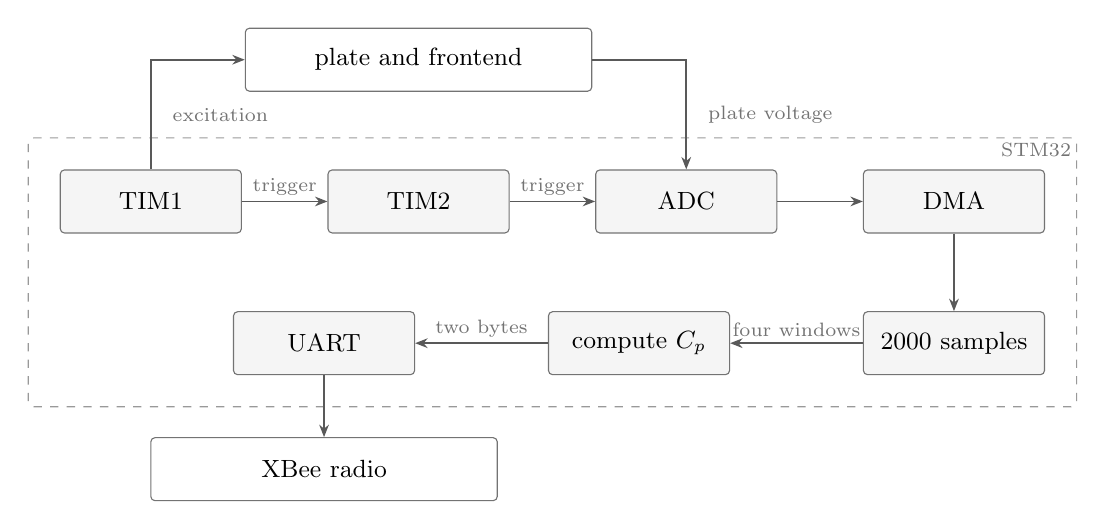
\begin{tikzpicture}[
  x=1mm, y=1mm, font=\small,
  blk/.style = {draw=black!55, fill=black!4, rounded corners=1.5pt,
                minimum width=23mm, minimum height=8mm, align=center,
                inner sep=3pt},
  ext/.style = {blk, fill=white, minimum width=44mm},
  ar/.style  = {-{Stealth[length=4.5pt,width=3.5pt]}, draw=black!65, semithick},
  lbl/.style = {font=\scriptsize, text=black!55, inner sep=2pt},
]

  % ---- external circuit -------------------------------------
  \node[ext] (fe)  at ( 34,  18) {plate and frontend};

  % ---- on-chip, acquisition ---------------------------------
  \node[blk] (t1)  at (  0,   0) {TIM1};
  \node[blk] (t2)  at ( 34,   0) {TIM2};
  \node[blk] (ad)  at ( 68,   0) {ADC};
  \node[blk] (dm)  at (102,   0) {DMA};

  % ---- on-chip, processing and output -----------------------
  \node[blk] (bf)  at (102, -18) {2000 samples};
  \node[blk] (cp)  at ( 62, -18) {compute $C_p$};
  \node[blk] (tx)  at ( 22, -18) {UART};

  % ---- radio ------------------------------------------------
  \node[ext] (xb)  at ( 22, -34) {XBee radio};

  % ---- arrows -----------------------------------------------
  \draw[ar] (t1) -- (t2) node[lbl, midway, above] {trigger};
  \draw[ar] (t2) -- (ad) node[lbl, midway, above] {trigger};
  \draw[ar] (ad) -- (dm);

  \draw[ar] (t1.north) |- (fe.west);
  \draw[ar] (fe.east) -| (ad.north);
  \node[lbl, anchor=west] at (  2, 11) {excitation};
  \node[lbl, anchor=west] at ( 70, 11) {plate voltage};

  \draw[ar] (dm) -- (bf);
  \draw[ar] (bf) -- (cp) node[lbl, midway, above] {four windows};
  \draw[ar] (cp) -- (tx) node[lbl, midway, above] {two bytes};
  \draw[ar] (tx) -- (xb);

  % ---- chip boundary ----------------------------------------
  \begin{scope}[on background layer]
    \node[draw=black!40, dashed, rounded corners=2pt, inner sep=4mm,
          fit=(t1)(dm)(bf)(tx)] (mcu) {};
  \end{scope}
  \node[lbl, anchor=north east] at (mcu.north east) {STM32};

\end{tikzpicture}
\caption{Acquisition path inside one node. The timers, ADC and DMA are chained in
hardware; the CPU only takes over once the frame is complete.}
\end{figure}

\vspace{-0.8em}
\section{Current state}

\begin{figure}[H]\centering
\begin{subfigure}[t]{0.48\textwidth}\centering
  \shot{matlab-results.png}{2.6cm}
  \caption{MATLAB output over successive rounds.}
\end{subfigure}
\hfill
\begin{subfigure}[t]{0.48\textwidth}\centering
  \shot{board-ok.jpg}{2.6cm}
  \caption{Complete board, as in the schematic.}
\end{subfigure}

\vspace{0.3em}

\begin{subfigure}[t]{0.48\textwidth}\centering
  \shot{board-r7-r3.jpg}{2.6cm}
  \caption{Board with R7 and R3 missing.}
\end{subfigure}
\hfill
\begin{subfigure}[t]{0.48\textwidth}\centering
  \shot{board-c1-r3.jpg}{2.6cm}
  \caption{Board with C1 and R3 missing.}
\end{subfigure}
\end{figure}

\vspace{-0.9em}
Two nodes report plausible capacitance. The others read implausibly high because
of the missing components shown above. Once those are repaired, the full
four-channel acquisition and the modelling that follows it can proceed.

\vspace{0.4em}
\hrule
\vspace{0.3em}
{\small Firmware, MATLAB server and full configuration reference:
\url{https://github.com/Erfan-TT/Capacitive_Sensor_Sync}}

\end{document}
